% !TeX program = pdflatex
\documentclass[tikz,border=8pt]{standalone}
\usepackage{tikz}\usetikzlibrary{positioning,arrows.meta}
\definecolor{FigureBlue}{HTML}{2563EB}\definecolor{FigureOrange}{HTML}{EA580C}\definecolor{FigureGreen}{HTML}{16A34A}
\begin{document}
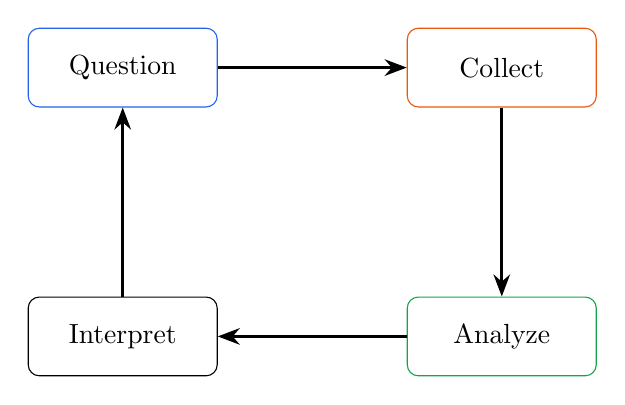
\begin{tikzpicture}[>=Stealth,node distance=24mm,every node/.style={draw,rounded corners,minimum width=24mm,minimum height=10mm,align=center}]
  \node[draw=FigureBlue] (q) {Question}; \node[draw=FigureOrange,right=of q] (c) {Collect};
  \node[draw=FigureGreen,below=of c] (a) {Analyze}; \node[below=of q] (i) {Interpret};
  \draw[->,line width=1.1pt] (q)--(c); \draw[->,line width=1.1pt] (c)--(a); \draw[->,line width=1.1pt] (a)--(i); \draw[->,line width=1.1pt] (i)--(q);
\end{tikzpicture}
\end{document}
